%%
%% Arquivo principal para:
%% - teses de doutorado
%% - dissertações de mestrado
%% - exames de qualificação de mestrado e doutorado
%%
%% NOTA: A PUBLICAÇÃO DESTE MODELO VISA APENAS ORIENTAR OS PÓS-GRADUANDOS
%% NA PREPARAÇÃO DE SEUS TEXTOS. O PPgEE DA UFRN NÃO PROVÊ ASSISTÊNCIA NO
%% USO DAS FERRAMENTAS NECESSÁRIAS AO USO DESTE MODELO (LATEX, XFIG, ETC.)
%%
%% Adelardo Medeiros, dezembro de 2005.

% DEFINIÇÕES GLOBAIS

% Esta primeira linha dá informações gerais sobre o documento.
% PARA A VERSÃO FINAL:
% papel A4, letra grande (12pt), openright (capítulos só iniciam em
% página direita, se necessário incluindo uma página em branco),
% twoside (o documento vai ser impresso em frente e costa)
\documentclass[a4paper,12pt,openright,twoside]{book}
% PARA A QUALIFICAÇÃO E PARA A VERSÃO INICIAL:
% papel A4, letra grande (12pt), openany (capítulos iniciam em
% qualquer página), oneside (o documento vai ser impresso só na frente)
%\documentclass[a4paper,12pt,openany,oneside]{book}

% PACOTES OBRIGATÓRIOS

% Use estes pacotes para poder digitar diretamente as letras com acento
% e para que a hifenização funcione corretamente
\usepackage[utf8]{inputenc}
\usepackage{ae}
% Para usar fontes standard ao invés das do LaTeX (gera melhores PDFs)
\usepackage{pslatex}
% Para a hifenização em português
\usepackage[portuges, brazil]{babel}
% Para que os primeiros parágrafos das seções também sejam indentados
\usepackage{indentfirst}
% Para poder incluir gráficos (figuras)
\usepackage{graphicx}
% Para poder fazer glossário ou lista de símbolos
% Use a segunda opção se quiser incluir na definição do símbolo a
% página e/ou a equação onde ela foi definida
\usepackage[portuguese,noprefix]{nomencl}
%\usepackage[portuguese,noprefix,refeq,refpage]{nomencl}
% Para permitir espaçamento simples, 1 1/2 e duplo
\usepackage{setspace}
% Para usar alguns comandos matemáticos avançados muito úteis
\usepackage{amsmath}
% Para poder usar o ambiente "comment"
\usepackage{verbatim}
% Para poder ter tabelas com colunas de largura auto-ajustável
\usepackage{tabularx}
% Para executar um comando depois do fim da página corrente
\usepackage{afterpage}
% Para formatar URLs (endereços da Web)
\usepackage{url}
% Para reduzir os espaços entre os ítens (itemize, enumerate, etc.)
% Este pacote não faz parte da distribuição padrão do LaTeX.
\usepackage{lib/noitemsep}
% Para as citações bibliográficas
\usepackage[alf]{abntex2cite}
%\usepackage[abbr]{lib/harvard}	% As chamadas são sempre abreviadas
%\harvardparenthesis{square}	% Colchetes nas chamadas
%\harvardyearparenthesis{round}	% Parêntesis nos anos das referências
%\renewcommand{\harvardand}{e}	% Substituir "&" por "e" nas referências

% PACOTES OPCIONAIS

% Para poder incluir arquivos Postscript com cores (do Xfig, por exemplo)
\usepackage{color}
% Para ter células em tabelas que ocupam mais de uma linha
\usepackage{multirow}
% Para poder ter tabelas longas em mais de uma página
%\usepackage{longtable}
% Para poder escrever partes do texto em "n" colunas
%\usepackage{multicol}
% Se você quiser personalizar os cabeçalhos das páginas
%\usepackage{fancyheadings}
% Para incluir algoritmos e listagens de códigos
%\usepackage{listings}
% Capítulos com títulos em um formato "decorado"
\usepackage{lib/capitulos}

% NOVOS COMANDOS

% As definições dos novos comandos estão agrupadas no arquivo "comandos.tex"
% Esta separação é opcional: se você preferir, pode por as definições
% diretamente neste arquivo
% newcommand define novos comandos, que podem passar a ser usados da
% mesma forma que os comandos LaTeX de base.

% Implicação em fórmulas
\newcommand{\implica}{\quad\Rightarrow\quad} %Meio de linha
\newcommand{\implicafim}{\quad\Rightarrow}   %Fim de linha
\newcommand{\tende}{\rightarrow}
\newcommand{\BibTeX}{\textsc{B\hspace{-0.1em}i\hspace{-0.1em}b\hspace{-0.3em}}\TeX}

% Fração com parentesis
\newcommand{\pfrac}[2]{\left(\frac{#1}{#2}\right)}

% Transformada de Laplace e transformada Z
%\newcommand{\lapl}{\makebox[0cm][l]{\hspace{0.1em}\raisebox{0.25ex}{-}}\mathcal{L}}
\newcommand{\lapl}{\pounds}
\newcommand{\transfz}{\mathcal{Z}}

% Não aparecer o número na primeira página dos capítulos
\newcommand{\mychapter}[1]{\chapter{#1}\thispagestyle{empty}}

% Os capítulos sem número
\newcommand{\mychapterast}[1]{\chapter*{#1}\thispagestyle{empty}
\chaptermark{#1}
\afterpage{\markboth{\uppercase{#1}}{\rightmark}}
\markboth{\uppercase{#1}}{}
}

% Seções sem número
\newcommand{\mysectionast}[1]{\section*{#1}
\addcontentsline{toc}{section}{#1}
\markright{\uppercase{#1}}
}

% No tabularx, as celulas devem ser centradas verticalmente
\renewcommand{\tabularxcolumn}[1]{m{#1}}

% Células centralizadas horizontalmente no tabularx
\newcolumntype{C}{>{\centering\arraybackslash}X}

%% Abrevia figuras e tabelas
%\def\figurename{Fig.}
%\def\tablename{Tab.}


%
% As margens
%

% Direção horizontal

% Margem interna
% Nas páginas ímpares
\setlength{\oddsidemargin}{3.5cm}         % Margem real desejada
% Nas páginas pares
\setlength{\evensidemargin}{2.5cm}        % Margem real desejada
% Largura do texto
\setlength{\textwidth}{15cm}
% As margens laterais no LaTeX são sempre 1 polegada maiores do que as
% fixadas. Se foi fixada \setlength{\oddsidemargin}{3.5cm}, a margem
% real seria de 3.5+2.54=6.04cm. Para permitir que você não tenha que
% fazer esta conta, pode usar o número desejado nas linhas anteriores
% e a gente subtrai 1in nas próximas linhas
\addtolength{\oddsidemargin}{-1in}
\addtolength{\evensidemargin}{-1in}
% Note que a margem direita não é fixada diretamente:
% ela é obtida subtraindo-se os outros valores da largura da página.
% 3.5+15+x=21cm (largura A4) -> x = margem externa = 2.5cm

% Direção vertical

% Margem superior (entre o topo da folha e o cabeçalho), altura do
% cabeçalho e distância entre o fim do cabeçalho e o início do texto
\setlength{\topmargin}{2.0cm}             % Margem real desejada
\setlength{\headheight}{1.0cm}
\setlength{\headsep}{1.0cm}
% Altura do texto (sem cabeçalho e rodapé)
\setlength{\textheight}{22.7cm}
% Distância do fim do texto ao rodapé
\setlength{\footskip}{1.0cm}
% A margem superior no LaTeX é sempre 1 polegada maior do que a
% fixada. Se foi fixada \setlength{\topmargin}{2.0cm}, a margem
%real seria de 2.0+2.54=4.54cm. Para permitir que você não tenha que
% fazer esta conta, pode usar o número desejado na linha anterior
% e a gente subtrai 1in na próxima linha
\addtolength{\topmargin}{-1in}
% Note que a margem inferior não é fixada diretamente:
% ela é obtida subtraindo-se os outros valores, sem incluir o
% "footskip", da altura da página.
% 2.0+1.0+1.0+22.7+x=29.7cm (altura A4) -> x = margem inferior = 3cm

%
% O estilo das referências bibliográficas
%

%\bibliographystyle{bib/ppgee}

%
% O espaçamento entre linhas
%

% As páginas iniciais são sempre em espaçamento simples
\singlespacing

% Para a criação do glossário (ou lista de símbolos)
\makenomenclature

% Lista de arquivos a serem processados. Estes comandos "includeonly" são
% dispensáveis e devem obrigatoriamente ser comentados na hora de gerar o
% documento definitivo. Eles servem para compilar apenas parte do documento.
% É útil, durante a redação, para que não se tenha de compilar todo o
% documento a cada vez que se faz uma alteração. Por exemplo, se eu estou
% fazendo alterações na dedicatória e as outras partes não têm interesse no
% momento, posso incluir (descomentar) a linha "\includeonly{preambulo}"
%\includeonly{rosto}
%\includeonly{catalograficos}
%\includeonly{preambulo}
%\includeonly{resumos}
%\includeonly{introducao/introducao}
%\includeonly{estilo/estilo}
%\includeonly{matematica/matematica}
%\includeonly{figuras/figuras}
%\includeonly{conclusao/conclusao}
%\includeonly{apendice/apendice}

% Inicia o texto
\begin{document}

% Paginas iniciais (sem numeração)
\pagestyle{empty}

% Página de rosto (capa interna)
%
% ********** P�gina de Rosto
%

% titlepage gera p�ginas sem numera��o
\begin{titlepage}

\begin{center}

\small

% O comando @{} no ambiente tabular x � para criar um novo delimitador
% entre colunas que n�o a barra vertical | que � normalmente utilizada.
% O delimitador desejado vai entre as chaves. No exemplo, n�o h� nada,
% de modo que o delimitador � vazio. Este recurso est� sendo usado para
% eliminar o espa�o que geralmente existe entre as colunas
\begin{tabularx}{\linewidth}{@{}l@{}C@{}r@{}}
% A figura foi colocada dentro de um parbox para que fique verticalmente
% centralizada em rela��o ao resto da linha
\parbox[c]{3cm}{
\includegraphics[width=\linewidth]{tex/00-estrutural/figuras/UFRN}} &
\begin{center}
\textsf{\textsc{Universidade Federal do Rio Grande do Norte\\
Centro de Tecnologia\\
Programa de P�s-Gradua��o em Engenharia El�trica}}
\end{center} &
\parbox[c]{2cm}{
\includegraphics[width=\linewidth]{tex/00-estrutural/figuras/PPgEE}}
\end{tabularx}

% O vfill � um espa�o vertical que assume a m�xima dimens�o poss�vel
% Os vfill's desta p�gina foram utilizados para que o texto ocupe
% toda a folha
\vfill

\LARGE

\textbf{Sobre a Prepara��o de Propostas de Tema, Disserta��es
e Teses no Programa de P�s-Gradua��o em Engenharia El�trica da UFRN}

\vfill

\Large

\textbf{Fulano dos Anz�is Pereira}

\vfill

\normalsize

Orientador: Prof. Dr. Sicrano Matosinho de Melo
% Se n�o houver co-orientador, comente a pr�xima linha
\\[2ex] Co-orientador: Prof. Dr. Beltrano Catandura do Amaral

\vfill

\hfill
\parbox{0.5\linewidth}{\textbf{%
% Descomente as op��es que se aplicam ao seu caso
%Proposta de Tema para Qualifica��o}
Disserta��o de Mestrado}
%Tese de Doutorado}
apresentada ao Programa de P�s-Gradua��o em Engenharia El�trica da UFRN
%(�rea de concentra��o: Automa��o e Sistemas)
(�rea de concentra��o: Engenharia de Computa��o)
%(�rea de concentra��o: Telecomunica��es)
como parte dos requisitos para obten��o do t�tulo de
Mestre em Ci�ncias.}
%Doutor em Ci�ncias.}

\vfill

\large

% Este n�mero de ordem deve ser obtido na coordena��o do PPgEE
% Corresponde ao n�mero seq�encial da sua tese ou disserta��o:
% por exemplo, a 25� tese de doutorado ter� o n�mero de ordem D25
% Evidentemente, este dado n�o existe para propostas de tema, caso
% em que a pr�xima linha deve ser comentada.
N�mero de ordem PPgEE: M000

Natal, RN, fevereiro de 2006

\end{center}

\end{titlepage}


% Ficha catalográfica: os dados catalográficos devem ser fornecidos
% pela BCZM.
% Só são incluídos na versão final da tese ou dissertação. Não são
% incluídos nem na proposta de tema de qualificação nem na versão
% preliminar da tese ou dissertação: nestes casos, comente a próxima linha.
%
% ********** Ficha Catalogr�fica
%

\newpage

\begin{center}

% Aqui n�o se usou \vfill porque o \vfill � constru�do internamente com
% o comando \vspace. Espa�os verticais no in�cio da folha com \vspace
% s�o ignorados. Para que isto n�o ocorra deve-se usar o \vspace*
% \vspace*{\fill} � como se fosse um \vfill*
\vspace*{\fill}

Divis�o de Servi�os T�cnicos\\[1ex]
Cataloga��o da publica��o na fonte.
UFRN / Biblioteca Central Zila Mamede

\vspace{2ex}

\begin{tabular}{|p{0.9\linewidth}|} \hline
\\
Pereira, Fulano dos Anz�is.\\
\hspace{1em} Sobre a Prepara��o de Propostas de Tema, Disserta��es
e Teses no Programa de P�s-Gradua��o em Engenharia El�trica da UFRN /
Fulano dos Anz�is Pereira - Natal, RN, 2006 \\
\hspace{1em} 23 p. \\
\\
\hspace{1em} Orientador: Sicrano Matosinho de Melo \\
\hspace{1em} Co-orientador: Beltrano Catandura do Amaral \\
\\
\hspace{1em} Tese (doutorado) - Universidade Federal do Rio Grande do Norte.
Centro de Tecnologia. Programa de P�s-Gradua��o em Engenharia El�trica. \\
\\
\hspace{1em} 1. Reda��o t�cnica - Tese. 2. \LaTeX - Tese.
I. Melo, Sicrano Matosinho de. II. Amaral, Beltrano Catandura do.
III. T�tulo. \\
\\
RN/UF/BCZM \hfill CDU 004.932(043.2) \\ \hline
\end{tabular} 

\end{center}


% Assinaturas da banca, dedicatória e agradecimentos
% Só são incluídos na versão final da tese ou dissertação. Não são
% incluídos nem na proposta de tema de qualificação nem na versão
% preliminar da tese ou dissertação: nestes casos, comente a próxima linha.
%
% ********** Página de assinaturas
%

\begin{titlepage}

\begin{center}

\LARGE

\textbf{Sobre a Preparação de Propostas de Tema, Dissertações
e Teses no Programa de Pós-Graduação em Engenharia Elétrica da UFRN}

\vfill

\Large

\textbf{Fulano dos Anzóis Pereira}

\end{center}

\vfill

% O \noindent é para eliminar a tabulação inicial que normalmente é
% colocada na primeira frase dos parágrafos
\noindent
% Descomente a opção que se aplica ao seu caso
% Note que propostas de tema de qualificação nunca têm preâmbulo.
Dissertação de Mestrado
%Tese de Doutorado
aprovada em 31 de fevereiro de 2006 pela banca examinadora composta
pelos seguintes membros:

% Os nomes dos membros da banca examinadora devem ser listados
% na seguinte ordem: orientador, co-orientador (caso haja),
% examinadores externos, examinadores internos. Dentro de uma mesma
% categoria, por ordem alfabética

\begin{center}

\vspace{1.5cm}\rule{0.95\linewidth}{1pt}
\parbox{0.9\linewidth}{%
Prof. Dr. Sicrano Matosinho de Melo (orientador) \dotfill\ DCA/UFRN}

\vspace{1.5cm}\rule{0.95\linewidth}{1pt}
\parbox{0.9\linewidth}{%
Prof. Dr. Beltrano Catandura do Amaral (co-orientador) \dotfill\ DCA/UFRN}

\vspace{1.5cm}\rule{0.95\linewidth}{1pt}
\parbox{0.9\linewidth}{%
Prof. Dr. Clint Stallone da Silva \dotfill\ DCEP/UFFN}

\vspace{1.5cm}\rule{0.95\linewidth}{1pt}
\parbox{0.9\linewidth}{%
Profª Drª Florisbela do Amaral \dotfill\ DCA/UFRN}

\end{center}

\end{titlepage}

%
% ********** Dedicatória
%

% A dedicatória não é obrigatória. Se você tem alguém ou algo que teve
% uma importância fundamental ao longo do seu curso, pode dedicar a ele(a)
% este trabalho. Geralmente não se faz dedicatória a várias pessoas: para
% isso existe a seção de agradecimentos.
% Se não quiser dedicatória, basta excluir o texto entre
% \begin{titlepage} e \end{titlepage}

\begin{titlepage}

\vspace*{\fill}

\hfill
\begin{minipage}{0.5\linewidth}
\begin{flushright}
\large\it
Aos meus filhos, Tico e Teco, pela paciência durante
a realização deste trabalho.
\end{flushright}
\end{minipage}

\vspace*{\fill}

\end{titlepage}

%
% ********** Agradecimentos
%

% Os agradecimentos não são obrigatórios. Se existem pessoas que lhe
% ajudaram ao longo do seu curso, pode incluir um agradecimento.
% Se não quiser agradecimentos, basta excluir o texto após \chapter*{...}

\chapter*{Agradecimentos}
\thispagestyle{empty}

\begin{trivlist}  \itemsep 2ex

\item Ao meu orientador e ao meu co-orientador, professores Sicrano
e Beltrano, sou grato pela orientação.

\item Ao professor Apolônio pela ajuda na revisão deste
modelo de tese.

\item Aos colegas Huguinho, Zezinho e Luizinho pelas sugestões de
modelos de tese.

\item Aos demais colegas de pós-graduação, pelas críticas e sugestões.

\item À minha família pelo apoio durante esta jornada.

\item À CAPES, pelo apoio financeiro.

\end{trivlist}


%
% O espaçamento entre linhas
%

% PARA A VERSÃO FINAL:
% Deve ser usado espaçamento simples nas páginas de texto
\singlespacing
% PARA A QUALIFICAÇÃO E PARA A VERSÃO INICIAL:
% Deve ser usado espaçamento 1 1/2 nas páginas de texto
%\onehalfspacing

% Resumo/Abstract
%
% ********** Resumo
%

% Usa-se \chapter*, e n�o \chapter, porque este "cap�tulo" n�o deve
% ser numerado.
% Na maioria das vezes, ao inv�s dos comandos LaTeX \chapter e \chapter*,
% deve-se usar as nossas vers�es definidas no arquivo comandos.tex,
% \mychapter e \mychapterast. Isto porque os comandos LaTeX t�m um erro
% que faz com que eles sempre coloquem o n�mero da p�gina no rodap� na
% primeira p�gina do cap�tulo, mesmo que o estilo que estejamos usando
% para numera��o seja outro.
\mychapterast{Resumo}

O resumo deve apresentar ao leitor uma id�ia compacta, mas clara do
trabalho descrito na tese. A defini��o precisa e import�ncia do
problema abordado, os principais objetivos, motiva��es e desafios da
pesquisa s�o bons pontos de partida para o resumo. A estrat�gia ou
metodologia empregada na pesquisa, suas principais contribui��es e os
resultados mais importantes tamb�m devem fazer parte do resumo. Note
que o resumo n�o deve ultrapassar uma p�gina.

\vspace{1.5ex}

{\bf Palavras-chave}: Processamento de texto, \LaTeX,
Prepara��o de Teses, Relat�rios T�cnicos.
%
% ********** Abstract
%

\mychapterast{Abstract}

The abstract must present to the reader a short, but clear idea of the
work being reported in the thesis. The precise definition and
importance of the problem being addressed, the main objectives,
motivations and challenges of the research are a good starting point
for the abstract. The strategy or metodology employed in the research,
its main contributions, and the most important results achieved may be
part of the abstract as well. Notice that the
abstract must not exceed one page.

\vspace{1.5ex}

{\bf Keywords}: Document Processing, \LaTeX, Thesis Preparation,
Technical Reports.


% Paginas introdutórias (com numeração romana)
\frontmatter

% Lista de conteúdo (sumário, gerado automaticamente)
\addcontentsline{toc}{chapter}{Sumário}
\tableofcontents

% Lista de figuras (gerada automaticamente)
\cleardoublepage
\addcontentsline{toc}{chapter}{Lista de Figuras}
\listoffigures

% Lista de tabelas (gerada automaticamente)
\cleardoublepage
\addcontentsline{toc}{chapter}{Lista de Tabelas}
\listoftables

% Glossário (gerado automaticamente - veja entradas em
% tex/00-introducao/introducao.tex e em tex/02-estilo/estilo.tex)
\cleardoublepage
\renewcommand{\nomname}{Lista de Símbolos e Abreviaturas}
\markboth{\MakeUppercase{\nomname}}{\MakeUppercase{\nomname}}
\addcontentsline{toc}{chapter}{\nomname}
% O argumento opcional do comando \printnomenclature é a largura deixada
% para os símbolos no glossário. Se seus símbolos são "largos", como
% neste exemplo,  é melhor por mais espaço do que o 1cm que é reservado
% por default
\printnomenclature[1.5cm]

% Páginas do texto principal (com cabeçalho)
\mainmatter
\pagestyle{headings}

% Para facilitar a organização, foi criado um diretório para cada
% capítulo do documento, pois assim os arquivos das figuras ficam
% classificados por capítulos

% Cap. 1 - Introdução
%%
%% Cap�tulo 1: Modelo de Cap�tulo
%%

% Est� sendo usando o comando \mychapter, que foi definido no arquivo
% comandos.tex. Este comando \mychapter � essencialmente o mesmo que o
% comando \chapter, com a diferen�a que acrescenta um \thispagestyle{empty}
% ap�s o \chapter. Isto � necess�rio para corrigir um erro de LaTeX, que
% coloca um n�mero de p�gina no rodap� de todas as p�ginas iniciais dos
% cap�tulos, mesmo quando o estilo de numera��o escolhido � outro.
\mychapter{Introdu��o}
\label{Cap:introducao}

Este documento � um modelo para propostas de tema para exames de
qualifica��o, disserta��es de mestrado e teses de doutorado a serem
submetidos ao Programa de P�s-Gradua��o em Engenharia El�trica (PPgEE)
da Universidade Federal do Rio Grande do Norte (UFRN).  Procure ler o
texto acompanhando o resultado produzido a partir do c�digo fonte que
o gerou.

Neste cap�tulo introdut�rio apresentaremos algumas id�ias gerais sobre
como compilar documentos utilizando o processador de textos \LaTeX.

\section{Processando textos com \LaTeX}

O \LaTeX\ n�o � um editor de texto no sentido convencional. Ele funciona
muito mais como um ``compilador'' de uma linguagem de programa��o de
textos:%
% Este � um comando para incluir um item no gloss�rio
% Note os % no fim da linha anterior e da pr�xima
\nomenclature{\LaTeX:}{um poderoso processador de textos}%
\begin{enumerate}
\item Inicialmente voc� escreve um ``programa'' nesta linguagem de
programa��o de textos (linguagem \LaTeX), dizendo o conte�do e a
formata��o do seu documento.  Para escrever este ``programa'' pode-se
usar qualquer editor de textos capaz de salvar documentos em formato
texto ASCII puro.
\item O pr�ximo passo � compilar este c�digo fonte, produzindo um arquivo
\texttt{.dvi} que funciona como um ``programa objeto''. Esta compila��o
� feita pelo programa \texttt{latex}.
\item Em seguida o arquivo \texttt{.dvi} � convertido para o formato no
qual se deseja produzir o texto: PostScript (usando o programa
\texttt{dvips}), PDF (usando o \texttt{pdflatex}, que j� faz esta fase
e a fase anterior) ou visualiza��o na tela (\texttt{xdvi}).
\end{enumerate}
Estas explica��es tomaram como base a vers�o do \LaTeX\ mais comum para
sistemas operacionais Unix. Existem outras implementa��es tanto para
Unix quanto para Windows, onde os comandos executados s�o diferentes
mas a id�ia geral � sempre a mesma.

Al�m do \texttt{latex} para compilar o texto, pode ser necess�rio
executar outros programas, como o \texttt{bibtex} para incluir
automaticamente as refer�ncias bibliogr�ficas ou o \texttt{makeindex}
para gerar o gloss�rio. Estes programas devem ser chamados em uma
ordem espec�fica. Para automatizar este processo, � fornecido um
arquivo \texttt{Makefile}, de modo que a compila��o completa pode
ser feita utilizando um dos seguintes comandos:%
\nomenclature{\BibTeX:}{uma ferramenta para gera��o autom�tica de
listas de refer�ncias bibliogr�ficas}%
\begin{description}
\item[{\tt make}:] executa a tarefa \emph{par default}, que pode ser
alterada no \texttt{Makefile} para apontar para qualquer uma das seguintes.
\item[{\tt make simples}:] apenas executa o \texttt{latex} uma vez;
\item[{\tt make principal.dvi}:] executa todos os passos e aplicativos
necess�rios para produzir o arquivo \texttt{.dvi} completo;
\item[{\tt make principal.ps}:] executa todos os passos e aplicativos
necess�rios para produzir o arquivo PostScript \texttt{principal.ps}
completo;
\item[{\tt make principal.pdf}:] executa todos os passos e aplicativos
necess�rios para produzir o arquivo PDF \texttt{principal.pdf} completo;
\item[{\tt make clean}:] remove todos os arquivos intermedi�rios gerados
no processo de compila��o, inclusive o \texttt{principal.dvi}.
\item[{\tt make realclean}:] al�m de fazer um \texttt{make clean}, remove
os arquivos \texttt{principal.ps} e \texttt{principal.pdf}.
\end{description}

\section{Organiza��o do texto}

O fecho do cap�tulo introdut�rio muitas vezes apresenta uma id�ia
global do trabalho, mostrando o que vai ser tratado nos cap�tulos
subseq�entes\footnote{Contrariando o que muitos acreditam, o trema
ainda n�o foi abolido do portugu�s oficial do Brasil, o que j�
aconteceu em Portugal; portanto, deve ser usado em palavras como
seq��ncia, freq��ncia e aq��fero.}.

Neste documento, o cap�tulo~\ref{Cap:estilo} apresenta as diretrizes
gerais sobre a formata��o dos textos. O cap�tulo~\ref{Cap:matematica}
apresenta alguns recursos dp \LaTeX\ para escrever express�es
matem�ticas, enquanto o cap�tulo~\ref{Cap:figuras} trata da inclus�o
de tabelas, gr�ficos e figuras no documento. O
cap�tulo~\ref{Cap:conclusao}, que faz as vezes de capitulo de
conclus�es e perspectivas, mostra alguns exemplos de constru��o
autom�tica de bibliografias utilizando o aplicativo \BibTeX\ e
menciona fontes adicionais para mais informa��es.




% Cap. 2 - Estilo
%%
%% Cap�tulo 2: Regras gerais de estilo
%%

\mychapter{Estilo}
\label{Cap:estilo}

Este cap�tulo apresenta considera��es de ordem geral sobre a
organiza��o que deve ser adotada no seu documento, tais como n�mero de
p�ginas, margens e subdivis�es.

\section{Dimens�es}
\label{Sec:estilo}

N�o h� um n�mero m�nimo ou m�ximo de p�ginas para propostas de tema,
disserta��es ou teses. Entretanto, se o seu documento for muito menor
do que a m�dia pode transmitir uma id�ia de falta de conte�do a
apresentar. Por outro lado, um documento muito grande corre o risco de
s� conseguir a aten��o total do leitor no seu in�cio, fazendo com que
as partes mais importantes, que geralmente est�o no final do
documento, n�o sejam devidamente consideradas. Apenas para servir como
par�metro, est�o indicados a seguir os limites usuais quanto ao n�mero
de p�ginas\footnote{Uma folha corresponde a uma p�gina em impress�o em
face simples e a duas p�ginas em impress�o em face dupla} dos
documentos do PPgEE da UFRN, adotando as margens e os espa�amentos
definidos neste modelo:
\begin{itemize}
\item Proposta de tema para exame de qualifica��o de mestrado:
entre 20 e 40 p�ginas
\item Proposta de tema para exame de qualifica��o de doutorado:
entre 30 e 50 p�ginas
\item Disserta��o de mestrado:
entre 50 e 100 p�ginas
\item Tese de doutorado:
entre 80 e 150 p�ginas
\end{itemize}

O tamanho padr�o para a fonte � de 12pt.  Para facilitar a escrita de
coment�rios, sugest�es e corre��es da banca, recomenda-se o espa�amento
1.5 entre as linhas do texto e a impress�o em um �nico lado da folhas
para os seguintes documentos:
\begin{itemize}
\item Proposta de tema para exame de qualifica��o;
\item Vers�o inicial de disserta��o de mestrado; e
\item Vers�o inicial de tese de doutorado.
\end{itemize}
Para as vers�es finais de teses e disserta��es, onde se busca uma
melhor qualidade visual e tipogr�fica do texto, deve-se utilizar
espa�amento simples entre as linhas e a impress�o nos dois lados da
p�gina.

As margens devem seguir os valores adotados neste documento, que podem
ser verificados no arquivo \texttt{principal.tex}. � importante notar
que, na vers�o final de teses ou disserta��es, recomenda-se a
impress�o nos dois lados da p�gina. Por esta raz�o, a margem direita
em p�ginas pares deve ter o mesmo valor que a margem esquerda em
p�ginas impares e vice-versa, para que a encaderna��o fique
correta. Tamb�m em raz�o da impress�o em frente e verso, os cap�tulos
devem sempre come�ar em uma p�gina de n�mero �mpar, com a eventual
inclus�o de uma p�gina em branco. O \LaTeX\ se encarrega de fazer
automaticamente estes ajustes.

\section{Divis�es do documento e refer�ncias cruzadas}
\label{Sec:divisoes}

Documentos do porte de uma tese ou disserta��o devem ser subdivididos
em cap�tulos. O cap�tulo deve conter uma introdu��o e um fecho.

A introdu��o do cap�tulo fornece ao leitor uma breve descri��o do que
ser� tratado no cap�tulo e n�o forma uma se��o: para exemplificar, a
introdu��o deste cap�tulo � o par�grafo que precede a primeira se��o.

O fecho do cap�tulo apresenta coment�rios finais sobre o que foi
desenvolvido no cap�tulo e/ou faz uma liga��o com o que ser� visto no
cap�tulo seguinte; normalmente � colocado em uma se��o espec�fica,
denominada ``Coment�rios Finais'', ``Conclus�es'', ``Resultados'',
``Avalia��o Final'' ou qualquer outra denomina��o que se adeque ao
texto.

Cap�tulos s�o divididos em se��es. O n�mero ideal de se��es �
imposs�vel de se precisar. Entretanto, um cap�tulo com uma �nica se��o
provavelmente deve ser agregado ao cap�tulo anterior ou posterior. Um
cap�tulo com quinze se��es provavelmente deve ser subdividido em dois
cap�tulos.

Cap�tulos, se��es e subse��es devem ser rotulados para que possam ser
referenciados em qualquer parte do texto.  Isto � feito com o comando
\verb|\label{}|, que deve ser colocado logo ap�s (nunca antes) o
comando que criou a se��o, cap�tulo, etc. O par�metro do comando
\texttt{label} � o nome simb�lico que ser� usado para se fazer
refer�ncia a esta entidade dentro do texto, com o comando
\verb|\ref{}|. O nome pode ser qualquer coisa, mas n�o pode conter
acentos, por exemplo. Neste documento n�s utilizamos a conven��o de
prefixar os r�tulos dos cap�tulos com \texttt{Cap:}, das se��es com
\texttt{Sec:}, das equa��es com \texttt{Eq:} e assim por diante, mas
esta conven��o n�o � obrigat�ria. Veja a seguir um exemplo de
utiliza��o das refer�ncias cruzadas:
% quotation � um ambiente para cita��es, que ficam "recuadas" em
% rela��o ao resto do texto
\begin{quotation}
\dots no cap�tulo~\ref{Cap:introducao} apresentamos um modelo de
cap�tulo de tese.
\end{quotation}
Note que, no c�digo fonte deste trecho de frase, o espa�o entre a palavra
\texttt{cap�tulo} e o comando \verb|\ref{}| foi escrito com
um \texttt{\~{}} e n�o com um espa�o normal. O \texttt{\~{}} � o
comando \LaTeX\ para criar um espa�o onde n�o se pode mudar de linha,
pois ficaria estranho se o texto ``no cap�tulo'' estivesse no fim de
uma linha e o n�mero \ref{Cap:introducao} no in�cio da outra linha.

Existe uma particularidade no c�digo fonte do par�grafo anterior. Para
se escrever:
\begin{quotation}
\dots o comando \LaTeX\ para criar\dots
\end{quotation}
se colocou depois do comando \verb|\LaTeX| um espa�o
precedido de uma contrabarra, ao inv�s de um espa�o normal. Isto porque
espa�os depois de comandos s�o ignorados pelo \LaTeX; com um espa�o
% Na linha anterior n�o houve necessidade do espa�o com contrabarra
% depois do comando \LaTeX, pois ele � seguido por um ; e n�o um espa�o
normal as palavras ficariam ligadas:
\begin{quotation}
\dots o comando \LaTeX para criar\dots
\end{quotation}
Ao inv�s do espa�o precedido pela contrabarra, poder-se-ia tamb�m
utilizar um \texttt{\~{}}. A diferen�a � que neste caso o \LaTeX\ n�o
poderia fazer uma quebra de linha entre as palavras.

\section{Se��es}
\label{Sec:secoes}  %% labels n�o devem conter caracteres acentuados

Se��es s�o divis�es do conte�do do cap�tulo. Esta divis�o
deve ser l�gica (tem�tica) e n�o f�sica (por tamanho).
Por exemplo, um cap�tulo que trata de \textit{software}
de sistema teria se��es que tratam de montadores, ligadores,
carregadores, compiladores e sistemas operacionais.

Tal como cap�tulos, se��es devem ser rotuladas para refer�ncia
em outras partes do texto. Se��es s�o divididas em subse��es.

\subsection{Subse��es}
\label{Sec:subsecoes}

Subse��es s�o divis�es de se��es. No exemplo do texto sobre
\textit{software} de sistema, a se��o referente a sistema operacional
conteria, por exemplo, subse��es que tratam de arquivos, processos,
mem�ria e entrada/sa�da.  Tal como se��es, subse��es s�o divis�es
tem�ticas do texto.

\subsubsection*{Subsubse��es}
\label{Sec:subsubsecoes}

Subsubse��es s�o divis�es de subse��es e n�o devem ser numeradas no
texto. O \texttt{*} ap�s o comando \texttt{subsubsection*} instrui
o \LaTeX\ a n�o numerar a subsubse��o. Esta mesma regra se aplica
a outros comandos. Por exemplo, \verb|\chapter{}|
inicia um cap�tulo, enquanto \verb|\chapter*{}|
inicia um cap�tulo sem n�mero. O comando \texttt{chapter*} foi
usado no arquivo \texttt{resumos.tex} para criar os cap�tulos n�o
numerados referentes ao resumo e ao \textit{abstract}.

\section{�ndices}

O \LaTeX\ � capaz de gerar automaticamente o �ndice do texto
(sum�rio), os �ndices de figuras e de tabelas e uma lista de s�mbolos
ou gloss�rio.

\subsection{Sum�rio}
\label{Sec:sumario}

Todas as divis�es numeradas (cap�tulos, se��es e subse��es) s�o
automaticamente inclu�das no sum�rio. Ao se criar uma nova divis�o �
necess�rio compilar duas vezes o texto com o \LaTeX: na primeira
compila��o ser� percebida a inclus�o da nova divis�o, enquanto na
segunda ser� gerado o �ndice atualizado. Esta mesma necessidade de uma
dupla compila��o aparece quando se acrescenta qualquer nova refer�ncia
cruzada: uma nova figura ou tabela, uma nova refer�ncia bibliogr�fica,
etc.

Al�m das divis�es que s�o inclu�das automaticamente no sum�rio, pode-se
incluir manualmente outras informa��es. Os �ndices, por exemplo, n�o
s�o inclu�dos automaticamente no sum�rio. Verifique no arquivo
\texttt{principal.tex} o que deve ser feito para fazer esta inclus�o.

\subsection{Listas de figuras e tabelas}
\label{Sec:listasfigtab}

Estas listas s�o geradas automaticamente a partir dos
\texttt{caption}'s de todos os ambientes \texttt{figure} e
\texttt{table}. Maiores detalhes sobre estes ambientes ser�o apresentados
no cap�tulo~\ref{Cap:figuras}.

\subsection{Lista de s�mbolos (gloss�rio)}
\label{Sec:glossario}

Este ambiente pode ser utilizado para produzir uma lista de s�mbolos,
um gloss�rio ou uma lista de abreviaturas. Ao utilizar pela primeira
vez uma entidade que precise de defini��o, o autor, ao final do
par�grafo, gera a entrada para o gloss�rio. A t�tulo de exemplo,
foram inclu�dos na lista alguns s�mbolos e abreviaturas que aparecem
no texto a seguir:

\begin{quotation}
As primeiras teses apresentadas no PPgEE da UFRN eram datilografadas
manualmente. Para escrever uma f�rmula simples como:%
\nomenclature[aa]{UFRN:}{Universidade Federal do Rio Grande do Norte}%
\nomenclature[az]{PPgEE:}{Programa de P�s-Gradua��o em Engenharia El�trica}%
\begin{equation}
\omega = \omega_0 + \alpha \cdot \Delta t
\label{Eq:glossario}
\end{equation}%
% H� problemas quando se p�e uma quebra de linha em um comando \nomenclature.
% Para evit�-lo, comenta-se com um % todos os fins de linha das linhas que
% cont�m o comando e da linha imediatamente anterior.
\nomenclature{$\omega$}{velocidade angular do corpo}%
\nomenclature{$\omega_0$}{velocidade angular inicial do corpo}%
\nomenclature{$\alpha$}{acelera��o angular do corpo}%
\nomenclature{$\Delta t$}{tempo decorrido desde o instante em que foi medida
a velocidade inicial at� o instante presente}%
os autores tinham que desenhar os s�mbolos manualmente ou, para os
mais afortunados, trocar in�meras vezes a esfera da sua m�quina de
datilografia.
\end{quotation}

A ordem de apari��o dos verbetes no gloss�rio � a seguinte:
inicialmente os s�mbolos, depois os n�meros e por �ltimo as
\textit{strings}. Voc� pode modificar esta ordem incluindo um
par�metro adicional no comando
\verb|\nomenclature[opcional]{simb}{signif}|. No exemplo, este
par�metro foi utilizado para colocar UFRN antes de PPgEE.

\section{Bibliografia}
\label{Sec:citacoes}

As refer�ncias bibliogr�ficas s�o inclu�das dentro de um ambiente
espec�fico para este fim, atrav�s dos comandos
\verb|\begin{thebibliography}| e \verb|\end{thebibliography}|. Um
documento s� pode conter um �nico destes ambientes. A refer�ncia aos
documentos no texto � feita usando-se refer�ncias cruzadas e chaves
simb�licas, da mesma forma que as equa��es e as figuras. Cada
documento dentro de um ambiente \texttt{thebibliography} � introduzido
por um comando \verb|\bibitem|. O argumento obrigat�rio (entre chaves)
do comando \texttt{bibitem} � a chave simb�lica pela qual o documento
ser� citado no texto, usando o comando \verb|\cite|.  O argumento
opcional (entre colchetes) do comando \texttt{bibitem} � a express�o
que ser� inserida tanto no texto, no local onde a refer�ncia foi
citada, quanto na lista de refer�ncias bibliogr�ficas, como etiqueta
do documento em quest�o.

O ambiente \texttt{thebibliography} pode ser digitado diretamente pelo
usu�rio ou gerado automaticamente a partir de um arquivo de
informa��es bibliogr�ficas. A digita��o manual tem a vantagem de
tornar o documento autocontido, enquanto a gera��o autom�tica permite
um melhor reaproveitamento das informa��es e uma maior uniformidade
das refer�ncias nos diversos documentos. Sempre que poss�vel,
aconselha-se a gera��o autom�tica, que � feita pelo aplicativo
\BibTeX.

A principal vantagem da gera��o autom�tica de bibliografias � que se
pode manter um arquivo �nico com todas as refer�ncias bibliogr�ficas
que foram ou podem vir a ser usadas em algum dos seus documentos
(artigos, tese, etc.).  O \BibTeX\ se encarrega de verificar quais
delas foram efetivamente citadas no documento sendo processado e gerar
um ambiente \texttt{thebibliography} que cont�m apenas os documentos
necess�rios.

As informa��es bibliogr�ficas devem ser salvas em um arquivo no
formato \BibTeX\ e com extens�o \texttt{.bib}. O formato \BibTeX\ 
permite referenciar diferentes tipos de documentos:
\begin{itemize}
\item artigos em revistas~\cite{art-solimaes03};
\item artigos em anais de simp�sios~\cite{proc-gates01};
\item artigos em colet�neas de artigos~\cite{col-pinto00};
\item cap�tulos de livros~\cite{inbook-santos00};
\item anais de simp�sios~\cite{proc-sbrc02};
\item livros~\cite{book-lamport94};
\item teses de doutorado~\cite{phd-gates01};
\item teses de mestrado~\cite{msc-santos03};
\item relat�rios t�cnicos~\cite{rep-omg2000};
\item manuais t�cnicos~\cite{man-orbix99};
\item trabalhos n�o publicados~\cite{unp-sichman02};
\item p�ginas na Internet~\cite{hp-novet03} (a data � o dia do
      �ltimo acesso � p�gina);
\item miscel�nea~\cite{misc-cruz03}.
\end{itemize}

O arquivo \BibTeX\ n�o cont�m nenhuma informa��o de formata��o. Esta
formata��o � definida atrav�s do comando \verb|\bibliographystyle|.
Este modelo inclui um arquivo de estilo (\texttt{ppgee.bst}) que gera
as refer�ncias no padr�o adotado para os documentos do PPgEE. Este
estilo � baseado no padr�o \texttt{jmr} do pacote \texttt{harvard}, com
as modifica��es necess�rias para a l�ngua portuguesa. Para maiores
informa��es, veja a documenta��o do pacote \texttt{harvard}, dispon�vel
na Internet ou na maiorias das instala��es \LaTeX.

A lista de refer�ncias bibliogr�ficas � gerada pelo comando
\verb|\bibliography|, cujo par�metro obrigat�rio � o nome do(s) arquivo(s)
que cont�m(�m) as informa��es bibliogr�ficas.  O \BibTeX\ se encarrega
de extrair deste(s) arquivo(s) as refer�ncias citadas, format�-las de acordo
com o estilo escolhido e gerar o ambiente \texttt{thebibliography}
correspondente. Este ambiente � salvo em um arquivo com termina��o
\texttt{.bbl}, que � automaticamente inserido no documento no local do
comando \verb|\bibliography|. Este procedimento pode ser melhor
compreendido analisando-se os arquivos \texttt{principal.tex} e
\texttt{bibliografia.bib}, al�m do arquivo \texttt{principal.bbl}
gerado automaticamente pelo \BibTeX.

Uma recomenda��o importante � que as cita��es n�o fazem parte do
texto; portanto, as frases devem fazer sentido mesmo que as express�es
de cita��o sejam removidas. Para exemplificar, n�o se deve usar:
\begin{quotation}
\dots conforme demonstrado por \cite{art-solimaes03}.
\end{quotation}
e sim:
\begin{quotation}
\dots conforme demonstrado por \citeasnoun{art-solimaes03}.

\dots conforme demonstrado na literatura
\citeaffixed{art-solimaes03}{e.g. }.\footnote{A abreviatura e.g.
significa por exemplo. Vem do latim \emph{exempli gratia}. Tamb�m se
usa, para o mesmo caso, v.g. (\emph{verbi gratia}) ou simplesmente
p.ex.}
\end{quotation}

\section{Considera��es finais}

Os simples fatos de utilizar corretamente uma boa ferramenta de
formata��o de textos e de seguir as recomenda��es quanto ao estilo
n�o garantem a qualidade do documento produzido. O principal
aspecto a ser levado em conta � a qualidade da reda��o.

Propostas de tema, disserta��es e teses devem ser escritas em
linguagem t�cnica, que difere em alguns aspectos da linguagem
liter�ria.  Em textos das ci�ncias exatas e tecnol�gicas, o objetivo
principal � a clareza e a corre��o, algumas vezes com um certo
preju�zo da est�tica liter�ria. Algumas recomenda��es quanto �
reda��o s�o as seguintes:
\begin{itemize}
\item Evite per�odos longos, reduzindo o n�mero de apostos, ora��es
subordinadas, pronomes relativos (o qual, que, cujo, o mesmo, do qual,
etc.) e invers�es na ordem normal de aparecimento dos elementos da
frase (sujeito, verbo, predicado). Divida per�odos longos em v�rias
frases menores, mesmo que seja necess�rio repetir alguns termos. Por
exemplo:
\begin{quotation}
\emph{Esta vers�o foi concebida por ocasi�o da disciplina de Sistemas
de Transmiss�o de Dados, que tinha como principal objetivo, fazer uso
de uma plataforma m�vel onde pudesse ser aplicada uma t�cnica de
transmiss�o de dados, possibilitando dessa forma o controle desta.}
\end{quotation}
pode ser substitu�do por:
\begin{quotation}
\emph{Esta vers�o foi concebida durante a disciplina de Sistemas de
Transmiss�o de Dados. O principal objetivo desta primeira vers�o
era aplicar uma t�cnica de transmiss�o de dados a uma plataforma
m�vel. O uso da t�cnica de transmiss�o de dados tornou poss�vel
o controle da plataforma m�vel.}
\end{quotation}
\item Verifique a pontua��o empregada para n�o separar por v�rgulas
o sujeito do verbo, como no exemplo anterior em ``\dots\emph{tinha
como principal objetivo, fazer uso de}\dots'', nem trocar pontos por
v�rgulas ou vice-versa. Estes erros geralmente aparecem associados a
per�odos muito longos, como nos dois exemplos a seguir:
\begin{quotation}
\emph{Quando a opera��o � realizada sem o sistema de recep��o, o
ve�culo se desloca e realiza tarefas, baseadas na programa��o do
dispositivo microcontrolador e leitura de sensores, como a odometria,
por exemplo, a tabela abaixo lista a fun��o atribu�da a cada pino.}
\end{quotation}
\begin{quotation}
\emph{A garra � dotada tamb�m de um conjunto de sensores mec�nicos
de fim de curso tipo contato seco normalmente aberto (NA), nas
posi��es de m�xima eleva��o e abertura, bem como dois sensores desse
mesmo tipo nas pin�as da garra que respondem a uma pequena press�o em
sua superf�cie, sendo respons�veis por pressionar o elemento objeto
que se deseja recolher. Evitando que o mesmo escorregue quando
erguido.}
\end{quotation}
\item Evite o uso de adjetivos que expressam julgamentos de valor de
maneira n�o quantific�vel. Por exemplo, ao inv�s de dizer que os
resultados foram excelentes, diga que em 98\% dos experimentos o erro
foi menor que 1\%, deixando ao leitor a tarefa de concluir se estes
resultados s�o excelentes ou n�o.
\end{itemize}

No que diz respeito aos recursos de formata��o, lembre-se que o
\LaTeX\ j� faz a maior parte do trabalho para voc�, seguindo padr�es
que foram definidos por especialistas para garantir uma boa qualidade
tipogr�fica. Portanto, tente n�o modificar ``manualmente'' a
formata��o gerada. Para isto, evite sempre que poss�vel os seguintes
recursos, pois um texto ``limpo'' � mais agrad�vel de ler que um texto
``enfeitado'':
\begin{itemize}
\item letras mai�sculas em palavras onde elas n�o t�m justificativa
gramatical: nomes de meses (janeiro e n�o Janeiro), apenas para dar
�nfase (\dots foi desenvolvido um Rob� M�vel com rodas\dots), etc.
\item \textbf{o uso indiscriminado de negrito;}
\item \textit{o uso de it�lico, exceto em palavras em outra l�ngua
ou em defini��es de termos que aparecem pela primeira vez;}
\item texto em fontes diferentes: \texttt{espa�amento uniforme}, \textsf{sem
serifa}, \textsc{caixa alta}, etc.
\item \underline{o uso de texto sublinhado;}
\item o uso excessivo de notas de rodap�\footnote{Notas de rodap�
s�o estas express�es no p� da p�gina.}.
\item palavras em l�ngua estrangeira quando existe uma equivalente
em portugu�s (desempenho e n�o \textit{performance}) ou neologismos
n�o justificados (downloadar, rand�mico, etc.)
\end{itemize}


% Cap. 3 - Matemática
%%
%% Cap�tulo 2: Express�es matem�ticas
%%

\mychapter{Express�es matem�ticas}
\label{Cap:matematica}

\LaTeX~� insuper�vel no processamento de express�es matem�ticas. Express�es
simples como $2^{n}$ podem ser editadas no pr�prio texto. Equa��es
complexas como:
% eqnarray � o comando LaTeX de base para express�es multilinhas com
% alinhamento. O & indica o ponto onde todas as linhas devem ser
% alinhadas. Neste cap�tulo ser�o apresentadas outras op��es de alinhamento
\begin{eqnarray} \label{eq:PDF:RSR}
  p \left( \gamma \right) & = & \frac{1}{2} \sqrt{\frac{M}{\gamma \bar{\gamma}_{b}}} \frac{1}{ \prod_{i=1}^M {\sqrt{\tilde{\gamma}_i}}}
  \int_0^{\sqrt{M \delta}} \int_0^{\sqrt{M \delta} - r_M } \cdots
  \int_0^{\sqrt{M \delta} - \sum_{i = 3}^M {r_i } } \nonumber \\
  & & p \left( {\frac{\sqrt{M \delta} - \sum_{i = 2}^M {r_i }}{\sqrt{\tilde{\gamma}_1}} ,
  \frac{r_2}{\sqrt{\tilde{\gamma}_2}} , \ldots ,\frac{r_M}{\sqrt{\tilde{\gamma}_M}} } \right)
  \, dr_2 \cdots dr_{M-1} \, dr_M
\end{eqnarray}
% sem linha em branco
ou:
% sem linha em branco
\begin{equation} \label{eq:TrCGI}
  T(r) = \frac{1}{f_m}
  \left( \frac{\pi}{2} \sum_{i=1}^M
  {\tilde{r}_i^2 \dot{\varsigma}_i^2}\right)^{-1/2}
  \frac
  {\begin{array}{ll}
  \int_0^{\rho \sqrt{M}} \int_0^{\rho \sqrt{M} - r_M } \cdots
  \int_0^{\rho \sqrt{M} - \sum_{i = 3}^M {r_i } } \int_0^{\rho \sqrt{M} -
  \sum_{i = 2}^M {r_i } }  \\
  p \left( {\frac{r_1}{\tilde{r}_1} ,
  \frac{r_2}{\tilde{r}_2} , \ldots ,\frac{r_M}{\tilde{r}_M} } \right)
  \, dr_1 \, dr_2 \cdots dr_{M-1} \, dr_M \\ \end{array}}
  {\begin{array}{ll}
  \int_0^{\rho \sqrt{M}} \int_0^{\rho \sqrt{M} - r_M } \cdots
  \int_0^{\rho \sqrt{M} - \sum_{i = 3}^M {r_i } } \\
  p \left( {\frac{\rho \sqrt{M} - \sum_{i = 2}^M {r_i }}{\tilde{r}_1} ,
  \frac{r_2}{\tilde{r}_2} , \ldots ,\frac{r_M}{\tilde{r}_M} } \right)
  \, dr_2 \cdots dr_{M-1} \, dr_M \\ \end{array}}
\end{equation}

% ops, aqui eu deixei uma linha em branco de prop�sito
s�o automaticamente numeradas e podem ser referenciadas a partir do
texto. Por exemplo, a equa��o~\ref{eq:TrCGI} � trivialmente derivada
da equa��o~\ref{eq:PDF:RSR}.

No par�grafo anterior foi intencionalmente introduzido um erro. Note
que o trecho de frase ``s�o automaticamente numeradas\dots'' tem uma
indenta��o, ou seja, um espa�o inicial de tabula��o, como se fosse a
primeira frase de um novo par�grafo. Na realidade, todo o texto
anterior constitui um �nico par�grafo, no meio do qual se inserem as
duas equa��es. Por esta raz�o, os trechos de frase ap�s as equa��es
n�o devem se iniciar com letra mai�scula nem ser indentados. �
importante lembrar que nestas situa��es em que frases s�o
interrompidas por equa��es � obrigat�ria a inclus�o de dois pontos no
fim dos trechos da frase, como em ``\dots Equa��es complexas como:'' e
em ``ou:''.

O que gerou este erro de indenta��o? Lembre-se que em \LaTeX\ uma
linha em branco no c�digo fonte indica a separa��o entre dois
par�grafos. A causa do problema � a linha em branco entre o
\verb|\end{equation}| e o \texttt{s�o automaticamente
numeradas}\dots~. Como regra geral, enquanto um par�grafo n�o for
encerrado, n�o podem ser inclu�das linhas em branco, mesmo que no meio
do par�grafo existam equa��es, figuras, notas de rodap�, etc.

Pequenas express�es matem�ticas como $x_0^2$ podem ser inseridas
diretamente no texto, delimitadas por cifr�es (\texttt{\$}). Deve-se
evitar este recurso com express�es muito grandes, como
% array � o ambiente para fazer coisas como matrizes. � muito similar
% ao tabular, que ser� explicado no pr�ximo cap�tulo, com a diferen�a
% que os elementos do array s�o express�es matem�ticas.
% Para fazer uma matriz , lembre-se que o array n�o inclui os
% delimitadores. No caso, n�s pusemos o array dentro de delimitadores
% \left[ e right]. Estes delimitadores desenham um colchete do tamanho
% necess�rio para incluir a coisa delimitada
$\left[\begin{array}{cc} 1 & \frac{2}{x+1} \\ -2 &
1\end{array}\right]^{-1}$, porque o espa�amento entre as linhas fica
prejudicado. Para incluir express�es n�o numeradas maiores, pode-se
utilizar o par de delimitadores \verb|\[| e \verb|\]|, o que gera
express�es centralizadas na p�gina:
\[
% Nesta express�o n�s trocamos o delimitador das matrizes, passando
% a usar par�nteses
\left(\begin{array}{cc}
1 & \frac{2}{x+1} \\ -2 & 1
\end{array}\right)^{-1} = \left(\begin{array}{cc}
\frac{x+1}{x+5} & -\frac{2}{x+5} \\ \frac{2(x+1)}{x+5} & \frac{x+1}{x+5}
\end{array}\right) \quad
% quad � uma das formas de incluir espa�o em express�es matem�ticas,
% pois os espa�os s�o ignorados. quad deve ser usado com modera��o,
% pois na maioria dos casos a formata��o do LaTeX � a mais adequada.
% Muitos usos de quad podem ser substitu�dos por ambientes de alinhamento,
% explicados a seguir
\text{se} \quad x \neq -1 \quad \text{e} \quad x \neq -5
\]

Um erro comum em express�es matem�ticas � o de digitar os nomes de
fun��es diretamente, sem utilizar os comandos apropriados. Por
exemplo, a express�o $\sin(\omega t+\phi)$ est� correta, enquanto que
a express�o $sin(\omega t+\phi)$ � interpretada pelo \LaTeX como sendo
o produto das vari�veis $s$, $i$ e $n$ pela express�o entre
par�nteses. Para as fun��es usuais j� existem comandos predefinidos,
como \verb|\sin|. Para suas pr�prias fun��es, utilize o comando
\verb|\operatorname{}|, diretamente ou definindo um novo comando:
% newcommand define novos comandos, que podem passar a ser usados da
% mesma forma que os comandos LaTeX de base.
\newcommand{\fat}{\operatorname{fatorial}}
\[
\fat(x) = x \cdot \fat(x-1)
\]

O \LaTeX\ possui uma sintaxe espec�fica para �ndices (sub-escritos) e
expoentes (super-escritos) posicionados do lado direito do objeto a
que se referem, mas n�o do lado esquerdo. Para conseguir este efeito,
adicione �ndices e/ou expoentes a um bloco vazio posicionado antes do
objeto:
% O ambiente xalignat* � normalmente utilizado para escrever express�es
% matem�ticas multilinhas com v�rios pontos de alinhamento. Ser� detalhado
% na pr�xima se��o. Neste caso, est� sendo usado de um modo n�o
% convencional, pois se trata de uma express�o s� com uma linha. O ambiente
% xalignat* est� sendo empregado aqui para espa�ar igualmente os 6 �tens
% da express�o ao longo da linha de texto.
\begin{xalignat*}{3}
    &w^2 &     &w_i &   {}_z&w \\
{}^*&w   & {}_P&w^Q & {}^A_B&w^C_D
\end{xalignat*}

\section{Equa��es}
\label{Sec:equacoes}

As equa��es s�o delimitadas por \verb|\begin{equation}| e
\verb|\end{equation}|. Devem ser identificadas por um \verb|\label|
para permitir refer�ncias futuras:
% Nesta equa��o s�o utilizados delimitadores. N�o se pode usar um
% delimitador direito sem o esquerdo correspondente, mas os delimitadores
% n�o precisam ser do mesmo tipo (posso abrir com chave e fechar com
% colchete, por exemplo). Existe o delimitador . que � um delimitador
% vazio. Para colocar uma barra vertical ao lado das express�es, colocamos
% um delimitador . � esquerda e um delimitador | � direita.
\begin{equation}
y = g(x) = g(x_{PO}) + \left.\frac{dg}{dx}\right|_{x=x_{PO}}
\frac{(x-x_{PO})}{1!} + \left.\frac{d^2g}{dx^2}\right|_{x=x_{PO}}
\frac{(x-x_{PO})^2}{2!} + \cdots
\label{Eq:Taylor}
\end{equation}

Devem-se evitar refer�ncias com express�es do tipo ``a equa��o acima''
e ``a pr�xima equa��o'', pois modifica��es no texto podem tornar a
refer�ncia inv�lida. Use sempre refer�ncias pelo r�tulo
(\texttt{label}), como em ``a equa��o~\ref{Eq:Taylor}'', mesmo para
equa��es pr�ximas.

Existem v�rios ambientes para escrever equa��es, como o \verb|cases|
para construir express�es condicionais:
\begin{equation}
f(x) = 1+\begin{cases}
0   & \text{se $x=0$}\\
1/x & \text{caso contr�rio}
\end{cases} + \begin{cases}
x/2             & \text{se $x$ � inteiro e par}\\
\frac{x+1}{2}   & \text{se $x$ � inteiro e �mpar}\\
\frac{x+0.5}{2} & \text{se $x$ n�o � inteiro}
\end{cases}
\end{equation}

\section{Express�es multilinhas}
\label{Sec:multilinhas}

O pacote \texttt{amstex} define v�rios ambientes para criar express�es
matem�ticas que ocupam mais de uma linha. Existem vers�es dos
ambientes com e sem inclus�o do n�mero na equa��o, conforme indicado
na tabela~\ref{Tab:multilinhas}\footnotemark.
% A explica��o sobre o comando \footnotemark est� logo mais � frente
% no texto

\begin{table}[htbp]
\begin{center}
\newlength{\LL}
\settowidth{\LL}{Tipo de alinhamento}
\begin{tabular}{|>{\tt}l|>{\tt}l|l|} \hline
\multicolumn{2}{|c|}{PACOTE} &
\multicolumn{1}{c|}{\multirow{2}{\LL}{Tipo de alinhamento}}
\\ \cline{1-2}
\textrm{Com n�mero} & \textrm{Sem n�mero} &  \\ \hline
gather & gather* & sem alinhamento (s� m�ltiplas linhas) \\
multiline & multline* & quebra de equa��o em v�rias linhas \\
align & align* & alinhamento em um �nico ponto \\
alignat & alignat* & alinhamento em v�rios pontos, no centro da linha\\
xalignat & xalignat* & v�rios pontos, ocupando toda a linha (com margens)\\
-- & xxalignat & v�rios pontos, ocupando toda a linha (sem margens)
\\ \hline
\end{tabular}
\end{center}
\caption{Os ambientes para gera��o de equa��es multilinhas}
\label{Tab:multilinhas}
\end{table}

Para os ambientes \texttt{alignat}, \texttt{xalignat} e
\texttt{xxalignat} existe um par�metro obrigat�rio que � o n�mero de
elementos em cada linha. Cada elemento tem um ponto de alinhamento com
os outros elementos da mesma coluna em outras linhas.  Cada elemento �
separado do pr�ximo por um \texttt{\&}. Dentro de cada elemento, um
novo \texttt{\&} marca seu ponto de alinhamento, conforme o exemplo da
tabela \ref{Tab:exemplomultilinhas}, onde se v� o c�digo fonte e o
resultado produzido.

% Este table n�o cont�m um tabular, mas sim uma frase composta por
% dois minipages. Maiores detalhes sobre tables, tabulars, etc. no
% cap�tulo seguinte.
\begin{table}[htbp] \begin{center}
\hrule
% O ambiente minipage cria uma microp�gina com a dimens�o especificada
% e que se comporta exatamente como a p�gina real, por�m com dimens�es
% reduzidas. Ela pode ser inclu�da em praticamente todo outro ambiente
% e no meio de frases.
\begin{minipage}[c]{0.3\linewidth}
\tiny
% O ambiente verbatim p�e na tela o texto exatamente como foi digitado.
% Muito �til para incluir c�digo fonte, como neste caso.
\begin{verbatim}
\begin{xxalignat}{3}
&aaaa  &  mm&mm  &  cccc& \\
xxxx&  &  ii&ii  &  llll&
\end{xxalignat}
\end{verbatim}
\end{minipage}
% para uma minipage ficar � esquerda e a outra � direita vamos
% incluir entre elas dois espa�os horizontais \hfill, que s�o espa�os
% que "esticam" at� ocupar a m�xima largura poss�vel.
\hfill
$\implica$
\hfill
\begin{minipage}[c]{0.3\linewidth}
\begin{xxalignat}{3}
% A primeira coluna alinha o in�cio de um com o fim do outro
% A segunda coluna alinha os dois pelo meio
% A terceira coluna alinha os dois pelo fim
&aaaa  &  mm&mm  &  cccc& \\
xxxx&  &  ii&ii  &  llll&
\end{xxalignat}
\end{minipage}
\hrule
\caption{Exemplo de equa��o multilinha com v�rios pontos de alinhamento}
\label{Tab:exemplomultilinhas}
\end{center}\end{table}

Os ambientes da tabela~\ref{Tab:multilinhas} funcionam como um
ambiente \texttt{equation}: ocupam toda a linha e centralizam a
express�o.  Em algumas situa��es, entretanto, se deseja incluir um
sub-ambiente multilinhas dentro de uma express�o mais geral. Para
isto, o \texttt{amstex} fornece as op��es listadas na
tabela~\ref{Tab:submultilinhas}\addtocounter{footnote}{-1}\footnotemark.
% Para inserir uma nota de rodap�, pode-se utilizar o comando \footnote,
% que j� insere a marca e o texto. Em algumas situa��es, entretanto, �
% preciso utilizar um comando para a marca (\footnotemark) e outro para
% o texto (\footnotetext). Uma das situa��es onde isto � necess�rio �
% o caso deste exemplo, onde queremos que duas marcas se refiram ao
% mesmo texto.
% O comando \footnotemark incrementa o contador das marcas de rodap�,
% de modo que o primeiro \footnotemark imprimir� a marca 1, o segundo a
% marca 2, etc. Para contornar este incremento autom�tico, n�s
% decrementamos o contador de uma unidade antes da segunda chamada.

% Agora vai o texto da nota de rodap�. Ele � associado � marca do
% �ltimo \footnotemark. O comando \footnotetext n�o incrementa o
% contador de notas de rodap�.
\footnotetext{Nestas tabelas foram utilizadas extens�es do ambiente
\texttt{tabular} fornecidas pelo pacote \texttt{tabularx}. Esta
extens�es ser�o explicadas no cap�tulo \ref{Cap:figuras}}

\begin{table}[htbp]
\begin{center}
\begin{tabular}{|>{\tt}l|l|} \hline
% Estes multicolumn's que abranjem uma �nica coluna s�o utilizados para
% mudar o tipo de alinhamento. Por default, a primeira coluna � alinhada
% � esquerda (l). Usando o multicolumn, consegue-se que apenas o elemento
% na linha em quest�o fique centralizado (c).
\multicolumn{1}{|c|}{PACOTE} &
\multicolumn{1}{c|}{Tipo de alinhamento}
\\ \hline
gathered & sem alinhamento (s� m�ltiplas linhas) \\
aligned & alinhamento em um �nico ponto \\
alignedat & alinhamento em v�rios pontos
\\ \hline
\end{tabular}
\end{center}
\caption{Os ambientes para gera��o de trechos multilinhas em equa��es}
\label{Tab:submultilinhas}
\end{table}

A equa��o \ref{Eq:alinhamento} ilustra a utiliza��o de ambientes
\texttt{aligned} inseridos dentro de um ambiente \texttt{alignat}.
Nos ambientes multilinhas numerados cada linha ter� seu pr�prio n�mero
e dever� receber seu pr�prio r�tulo (\texttt{label}), exceto caso se
informe explicitamente que a linha n�o dever� ser numerada, usando o
comando \verb|\nonumber|.

\begin{alignat}{3}
% Primeira linha do alignat (n�o numerada)
% Primeiro elemento do alignat (inclui um aligned) - alinha no fim
\left\{\begin{aligned} % Alinha no sinal de =
\dot{\mathbf{x}}(t) &= \mathsf{A}\mathbf{x}(t)+\mathsf{B}\mathbf{u}(t) \\
\mathbf{y} &= \mathsf{C}\mathbf{x}(t)+\mathsf{D}\mathbf{u}(t)
\end{aligned}\right.&
% Note que o aligned � envolvido por dois delimitadores diferentes:
% uma chave (\left\{) no lado esquerdo e um vazio (\right.) no direito
&
% Segundo elemento do alignat (s� uma seta) - alinha no in�cio
&\implica
&
% Terceiro elemento do alignat (inclui um aligned) - alinha no in�cio
&\left\{\begin{aligned} % Alinha no sinal de =
s\mathbf{X}(s)-\mathbf{x}(0)&=\mathsf{A}\mathbf{X}(s)+\mathsf{B}\mathbf{U}(s)\\
\mathbf{Y}(s) &= \mathsf{C}\mathbf{X}(s)+\mathsf{D}\mathbf{U}(s)
\end{aligned}\right.\implicafim
\nonumber
\\
% Segunda linha do alignat (numerada)
% Primeiro elemento do alignat (inclui um aligned) - alinha no fim
\left\{\begin{aligned} % Alinha no sinal de =
\mathbf{X}(s) &= \Phi(s)\mathbf{x}(0) + \Phi(s)\mathsf{B}\mathbf{U}(s) \\
\mathbf{Y}(s) &= \mathsf{C}\mathbf{X}(s)+\mathsf{D}\mathbf{U}(s)
\end{aligned}\right.&
&
% Segundo elemento do alignat - alinha no in�cio
&\quad \text{onde} \quad
&
% Terceiro elemento do alignat - alinha no in�cio
&\Phi(s) = (s\mathsf{I}-\mathsf{A})^{-1}
\label{Eq:alinhamento}
\end{alignat}


% Cap. 4 - Figuras, gráficos e tabelas
%%
%% Cap�tulo 4: Figuras, gr�ficos e tabelas
%%

\mychapter{Figuras, tabelas e gr�ficos}
\label{Cap:figuras}

Uma das maiores dificuldades na edi��o de textos de qualidade � o
posicionamento dos elementos gr�ficos: figuras, gr�ficos e
tabelas. Como estes elementos muitas vezes s�o grandes, aparece o
dilema sobre o que fazer quando uma quebra de p�gina deveria acontecer
no meio do elemento. H� duas possibilidades:
\begin{enumerate}
\item O autor informa exatamente onde o elemento gr�fico deve ficar no
texto, evitando que quebras de p�ginas aconte�am no meio de um
elemento. O problema com esta abordagem � que todo o trabalho de
posicionamento pode ser perdido caso se inclua ou se exclua algum
texto ou elemento.
\item O editor de texto posiciona os elementos gr�ficos de forma a n�o
deixar espa�os em branco nas p�ginas. Estes elementos que podem ser
posicionados pelo editor s�o conhecidos como \emph{elementos
flutuantes}. O problema com esta abordagem � que o posicionamento
adotado pode n�o corresponder �s expectativas do autor.
\end{enumerate}

O \LaTeX\ oferece as duas possibilidades de posicionamento. Este
cap�tulo apresenta exemplos de inclus�o de elementos gr�ficos no
texto, bem como algumas ferramentas externas ao \LaTeX\ que podem ser
utilizadas para ger�-los.

\section{Elementos flutuantes}
\label{Sec:flutuantes}

Para caracterizar uma parte do texto como sendo flutuante, ela deve ser
delimitada por \verb|\begin{figure}| e \verb|\end{figure}| ou por
\verb|\begin{table}| e \verb|\end{table}|. Apesar do que os nomes
sugerem, nada obriga que o ambiente \texttt{figure} seja usado para
delimitar figuras ou que o ambiente \texttt{table} seja usado para
delimitar tabelas, embora esta seja a escolha quase sempre
adotada. Estes dois ambientes s�o praticamente equivalentes, com as
seguintes diferen�as:
\begin{itemize}
\item os dois ambientes usam contadores diferentes para numerar os
elementos flutuantes;
\item os ambientes \texttt{figure} ser�o inclu�dos na
\texttt{listoffigures}, enquanto os ambientes \texttt{table} ser�o
inclu�dos na \texttt{listoftables};
\item as legendas (\texttt{caption}'s) dos ambientes \texttt{figure}
ser�o precedidas da palavra ``Figura \dots'', enquanto as legendas dos
ambientes \texttt{table} ser�o precedidas da palavra ``Tabela \dots''.
Estas duas palavras podem ser alteradas pelo autor.
\end{itemize}
Para ilustrar o fato de que estes ambientes podem conter virtualmente
qualquer coisa, a figura~\ref{Fig:textoflutuante} cont�m um texto que
foi tornado flutuante por ser inclu�do em um ambiente \texttt{figure}
e as tabelas \ref{Tab:equacaoflutuante} e \ref{Tab:equacaoflutuante2}
cont�m express�es matem�ticas flutuantes, inclu�das em um ambiente
\texttt{table}. A tabela (\texttt{table}) \ref{Tab:submultilinhas} na
p�gina \pageref{Tab:submultilinhas} tamb�m n�o cont�m uma tabela no
sentido estrito do termo, mas sim uma linha de texto formada por duas
\texttt{minipage}'s separadas por um espa�o horizontal. A primeira
\texttt{minipage} cont�m um trecho de c�digo fonte e a segunda, o
resultado produzido (uma express�o matem�tica multialinhada).

\begin{figure}[tbp]
\caption{Trecho de \emph{Os Lus�adas}, de Luis de Cam�es}
\label{Fig:textoflutuante}
% hrule - linha horizontal
\hrule
% As minipage's s�o muito �teis para se colocar duas coisas na mesma linha
\begin{minipage}{0.45\linewidth}
% flushleft - alinha � esquerda
\begin{flushleft}
As armas e os bar�es assinalados\\
Que da ocidental praia lusitana\\
Por mares nunca dantes navegados\\
Passaram ainda al�m da Trapobana\\
Em perigos e guerras esfor�ados\\
Mais do que prometia a for�a humana\\
Entre gente remota edificaram\\
Novo reino, que tanto sublimaram
\end{flushleft}
\end{minipage}
\hfill
\begin{minipage}{0.45\linewidth}
% flushright - alinha � direita
\begin{flushright}
E tamb�m as mem�rias gloriosas\\
Daqueles reis que foram dilatando\\
A F�, o Imp�rio, as terras viciosas\\
De �frica e �sia andaram devastando,\\
E aqueles que por obras valerosas\\
Se v�o da lei da morte libertando:\\
Cantando espalharei por toda parte,\\
Se a tanto me ajudar o engenho e arte.
\end{flushright}
\end{minipage}
\hrule
\end{figure}

\begin{table}[bp]
% As minipage's s�o muito �teis para se colocar duas coisas na mesma linha
\begin{minipage}[b]{0.45\linewidth}
\begin{center}
\[
ax^2 + bx + c = 0
\]
\end{center}
\caption{Equa��o de segundo grau}
\label{Tab:equacaoflutuante}
\end{minipage}
\hfill
\begin{minipage}[b]{0.50\linewidth}
\begin{center}
\[
x = \frac{-b\pm\sqrt{b^2-4ac}}{2a}
\]
\end{center}
\caption{Ra�zes da equa��o da tabela~\ref{Tab:equacaoflutuante}}
\label{Tab:equacaoflutuante2}
\end{minipage}
\end{table}

� importante ressaltar que o que � numerado � o \texttt{caption} e n�o
a \texttt{figure} ou a \texttt{table}. Portanto, o \texttt{label} deve
ser colocado sempre ap�s o \texttt{caption} ao qual ele se
refere. Conforme ilustram as tabelas \ref{Tab:equacaoflutuante} e
\ref{Tab:equacaoflutuante2}, uma mesma \texttt{figure} ou
\texttt{table} pode ter mais de um ou nenhum \texttt{caption}.
O \texttt{caption} pode ser colocado antes do conte�do flutuante, como
na figura \ref{Fig:textoflutuante}, ou depois, como nas tabelas
\ref{Tab:equacaoflutuante} e \ref{Tab:equacaoflutuante2}. Nos
documentos do PPgEE, o padr�o � sempre posicionar o \texttt{caption}
abaixo das figuras e das tabelas.

\subsection{Posicionamento dos elementos flutuantes}
\label{Sec:posicionamento}

Em cada \verb|\begin{figure}| ou \verb|\begin{table}| pode-se incluir
um par�metro opcional com as op��es de posicionamento para este
elemento flutuante. Par�metros adicionais de comandos \LaTeX\ s�o
sempre fornecidos entre colchetes \texttt{[]}, enquanto os par�metros
obrigat�rios aparecem entre chaves \verb|{}|. As op��es dispon�veis
incluem as seguintes:
\begin{itemize}
\item[\tt h] O elemento pode ser posicionado na mesma posi��o em que ele
aparece no c�digo fonte do texto.
\item[\tt t] O elemento pode ser posicionado no topo de uma p�gina.
\item[\tt b] O elemento pode ser posicionado no fim de uma p�gina.
\item[\tt p] O elemento pode ser inclu�do em uma p�gina formada s� por
flutuantes.
\item[\tt !] Normalmente o \LaTeX\ faz algumas considera��es de ordem
est�tica no posicionamento dos flutuantes, o que �s vezes faz com que
alguns elementos sejam posicionados muito longe de onde s�o citados,
principalmente se voc� n�o incluir a op��o \texttt{p}. Para fazer com
que as considera��es est�ticas n�o sejam levadas em conta para um dado
elemento, inclua a op��o \texttt{!}.
\end{itemize}

\section{Tabelas em \LaTeX}
\label{Sec:tabelas}

Tabelas s�o constru�das com comandos pr�prios do \LaTeX, notadamente o
ambiente \texttt{tabular}. Nada obriga a que o ambiente
\texttt{tabular} esteja sempre posicionado em um elemento
flutuante. Se voc� quiser impor que uma tabela fique obrigatoriamente
em uma determinada posi��o do texto, basta n�o colocar o
\texttt{tabular} dentro de um \texttt{table}. Tabelas podem at� ser
inclu�das no meio de uma frase.  Por exemplo, eu posso dizer que se um
jogo da velha est� na configura��o \textsf{\tiny\begin{tabular}{c|c|c}
x & & x \\ \hline & & o \\ \hline x & o & \end{tabular}} e se o
jogador ``\textsf{x}'' sabe jogar, ent�o o jogador ``\textsf{o}'' ir�
perder, independentemente da jogada que fa�a.

O ambiente \texttt{tabular} tem um par�metro obrigat�rio que indica o
n�mero de colunas da tabela e o posicionamento dos objetos em cada
coluna. Por exemplo, uma tabela criada com \verb|\begin{tabular}{lcr}|
ter� tr�s colunas; o texto ser� alinhado � esquerda na primeira
coluna, centralizado na segunda e alinhado � direita na
terceira. Podem ser inclu�dos objetos que ocupam mais de uma linha
(comando \texttt{multirow}) ou mais de uma coluna (comando
\texttt{multicolumn}). Neste �ltimo caso, tamb�m � poss�vel mudar o
alinhamento do texto. Exemplos podem ser vistos nas tabelas
\ref{Tab:multilinhas} e \ref{Tab:submultilinhas}, na
p�gina~\pageref{Tab:multilinhas}.

Com o pacote \texttt{tabularx}, al�m das op��es normais de
posicionamento de colunas (\texttt{lcr}), pode-se incluir
automaticamente um texto qualquer antes de cada elemento da coluna
(\verb|>{}|). Este recurso foi utilizado nas tabelas
\ref{Tab:multilinhas} e \ref{Tab:submultilinhas} para fazer
com que todos os textos de algumas colunas fossem automaticamente
escritos na fonte \texttt{tt}. Al�m disso, podem-se criar colunas de
largura fixa e/ou de largura que se ajustam para que a tabela ocupe
toda a largura desejada, al�m do estilo tradicional de coluna que
assume a largura suficiente para conter seus elementos. Exemplos de
colunas com diferentes larguras e alinhamentos podem ser vistos na
tabela \ref{Tab:larguracolunas}.

\begin{table}[htbp]
\begin{tabularx}{\linewidth}{|p{3cm}|X|l|} \hline
COLUNA p & COLUNA X & COLUNA l \\ \hline
Largura fixa (n�o depende do conte�do) &
Expand�vel &
Ajust�vel \\ \hline
Alinhada no topo &
Alinhada � esquerda &
Alinhada � esquerda \\ \hline
\end{tabularx}
\\[0.5cm]
\begin{tabularx}{\linewidth}{|b{3cm}|C|r|} \hline
COLUNA b & COLUNA C (ver \texttt{comandos.tex}) & COLUNA r \\ \hline
Largura fixa (n�o depende do conte�do) &
Expand�vel &
Ajust�vel \\ \hline
Alinhada na base &
Centralizada &
Alinhada � direita \\ \hline
\end{tabularx}
\caption{Tabelas com colunas de diferentes larguras e alinhamentos}
\label{Tab:larguracolunas}
\end{table}

\section{Figuras em \LaTeX}
\label{Sec:figuras}

As figuras (imagens, desenhos, gr�ficos, etc.) devem ser produzidas
por ferramentas externas ao \LaTeX, salvas em um arquivo e inseridas
no texto usando o comando \texttt{includegraphics}. Da mesma forma
que as tabelas, as figuras podem ser flutuantes, caso sejam
inseridas dentro de um ambiente \texttt{figure}, ou ter uma posi��o
fixa no texto (como aqui: \includegraphics{tex/04-figuras/figuras/eu}).

O formato em que voc� deve salvar os arquivos das figuras para que
possa inclu�-las no texto depende de como voc� pretende compilar
o c�digo fonte:
\begin{itemize}
\item se o texto vai ser compilado com \texttt{latex}, todos os
arquivos devem estar no formato EPS (\emph{Encapsulated PostScipt});
\item se o texto vai ser compilado com \texttt{pdflatex}, os
arquivos devem estar nos formatos PDF ou JPEG (outros formatos s�o
aceitos, mas estes s�o os recomend�veis).
\end{itemize}
� aconselh�vel que voc� n�o inclua a termina��o no nome do arquivo que
� par�metro para o comando \texttt{includegraphics}. Isto porque, de
acordo com a forma como o texto est� sendo compilado, o \LaTeX\
acrescenta a termina��o adequada. Por exemplo, caso seu texto inclua o
comando \verb|\includegraphics{eu}|, o \LaTeX\ procurar� o arquivo
\texttt{eu.eps} caso esteja sendo chamado via \texttt{latex} ou um dos
arquivos \texttt{eu.pdf} ou \texttt{eu.jpg} caso esteja sendo chamado
via \texttt{pdflatex}.

As figuras podem ser divididas em dois grandes grupos:
\begin{itemize}
\item As imagens e fotos, que normalmente correspondem a vis�es reais
do mundo e s�o obtidas por c�meras digitais ou
assemelhados. Caracterizam-se por conterem grandes quantidades de
nuances, texturas e cores.
\item As figuras sint�ticas, normalmente produzidas utilizando
\emph{softwares} dedicados. Geralmente cont�m figuras geom�tricas
(linhas, quadrados, etc.), textos e poucas cores e texturas. Neste
grupo, para efeito de discuss�o das ferramentas de produ��o, podem-se
identificar duas categorias:
\begin{itemize}
\item Os desenhos e esquemas: diagramas de blocos, organogramas e
fluxogramas, representa��es esquem�ticas, etc.
\item Os gr�ficos: representa��es gr�ficas de valores ou fun��es
matem�ticas.
\end{itemize}
\end{itemize}

\subsection{Imagens e fotos}
\label{Sec:imagens}

As imagens e fotos normalmente s� podem ser armazenadas em formatos
que representam cada \emph{pixel} da imagem separadamente,
eventualmente com algum tipo de compress�o. Os formatos JPEG, GIF,
TIF, PNM (PBM, PGM ou PPM), BMP (Bitmap) e PNG, entre outros, s�o
todos desta categoria.  Se sua figura est� em algum destes formatos,
voc� deve convert�-la para EPS (se usar \texttt{latex}) ou para JPEG
(se usar \texttt{pdflatex}) para poder inclu�-la no documento \LaTeX.

A quase totalidade dos \emph{softwares} de visualiza��o de imagens
permite salv�-las em m�ltiplos formatos, geralmente incluindo JPEG e
EPS. No Unix, voc� disp�e ainda de v�rios programas para fazer a
convers�o em comandos de linha: \texttt{jpegtopnm},
\texttt{pnmtojpeg}, \texttt{pnmtops}, \texttt{gif2ps},
\texttt{giftopnm}, \texttt{tiff2ps}, \texttt{tifftopnm},
\texttt{bmptopnm} e \texttt{pngtopnm}, entre outros.

A figura \ref{Fig:belmonte} mostra um exemplo de inclus�o de uma
imagem no texto \LaTeX.

\begin{figure}[htbp!] \begin{center}
% fbox faz uma borda ao redor do seu argumento
\fbox{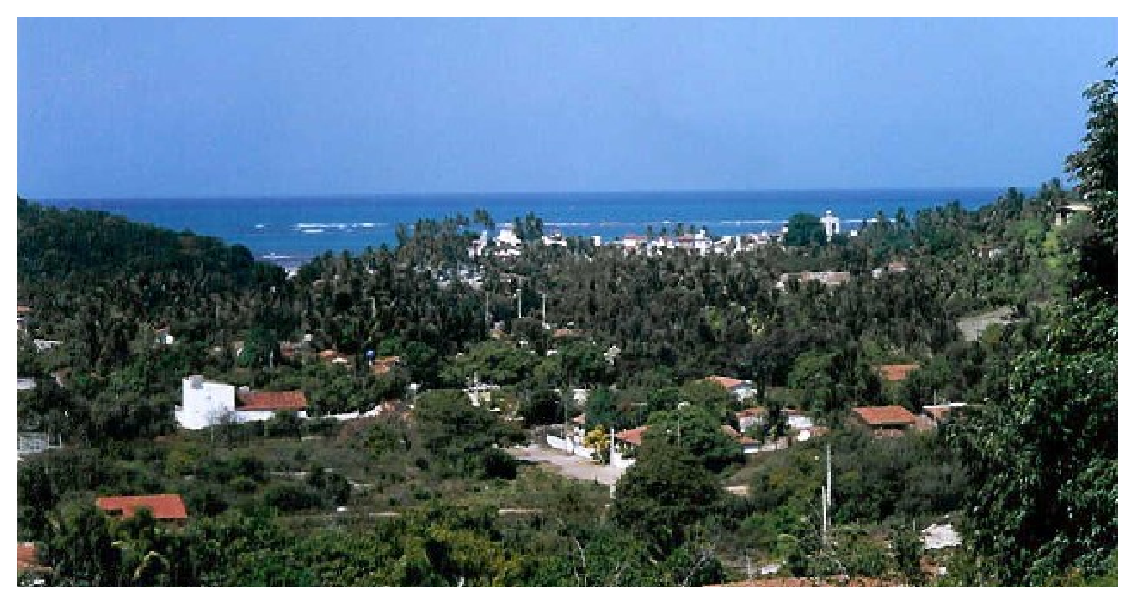
\includegraphics[width=0.75\linewidth]{tex/04-figuras/figuras/belmonte}}
\caption{Exemplo de imagem real}
\label{Fig:belmonte}
\end{center} \end{figure}

\subsection{Figuras sint�ticas}
\label{Sec:figsinteticas}

As figuras sint�ticas podem ser armazenadas em formato
\emph{pixel}-a-\emph{pixel}, como se fossem uma imagem, ou em
formato vetorial. No formato vetorial as primitivas que formam a
figura (linhas, textos, etc.) s�o descritas pelos par�metros que as
caracterizam (ponto de in�cio e fim, \emph{string} e posi��o do texto,
etc.). As figuras em formato vetorial s�o mais adequadas pois
usualmente correspondem a arquivos menores e a qualidade da imagem
n�o sofre perdas ao se aumentar ou diminuir o tamanho da figura.

Para inclus�o no \LaTeX, os formatos PDF e EPS s�o os �nicos que podem
representar figuras no formato vetorial. Nem toda figura salva nestes
formatos, entretanto, � necessariamente vetorial, pois tanto o PDF
quanto o EPS podem representar tanto figuras em formato
\emph{pixel}-a-\emph{pixel} quanto figuras em formato vetorial. Para
que sua figura seja vetorial, � necess�rio que o \emph{software} que a
gerou tenha a capacidade de produzi-las.

Para demonstrar a melhor qualidade das figuras em formato vetorial,
nas figuras \ref{Fig:bigvetorial} e \ref{Fig:bigbitmap} se mostra em
tamanho natural um mesmo diagrama nos formatos vetorial e de
\emph{pixels}. Nas figuras \ref{Fig:bigvetorialreduzida} e
\ref{Fig:bigbitmapreduzida} estas mesmas figuras s�o apresentadas
com uma redu��o de 50\%, utilizando o par�metro \texttt{scale} do
\texttt{includegraphics}. J� nas figuras \ref{Fig:smallvetorial} e
\ref{Fig:smallbitmap} o diagrama original foi reduzido, de forma que
seu tamanho natural � menor. Nas figuras
\ref{Fig:smallvetorialampliada} e \ref{Fig:smallbitmapampliada}
este diagrama pequeno est� aumentado de um fator arbitr�rio, calculado
pelo \texttt{includegraphics} para que a imagem ocupe toda a largura
da linha.

\begin{figure}[htbp!] \begin{center}
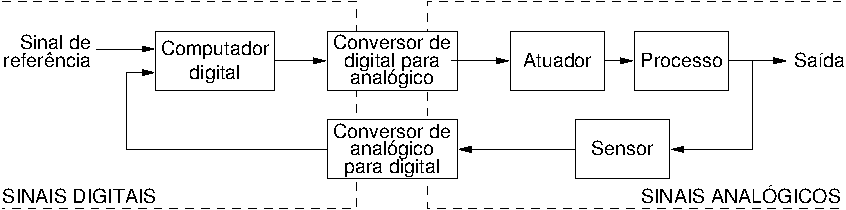
\includegraphics{tex/04-figuras/figuras/bigvetorial}
\caption{Figura vetorial grande em tamanho natural}
\vspace{6mm}
\label{Fig:bigvetorial}
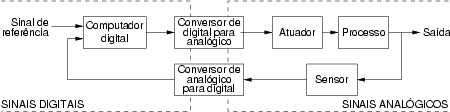
\includegraphics{tex/04-figuras/figuras/bigbitmap}
\caption{Figura \emph{pixel}-a-\emph{pixel} grande em tamanho natural}
\label{Fig:bigbitmap}
\vspace{6mm}
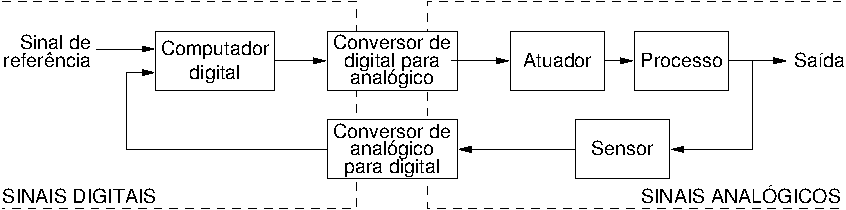
\includegraphics[scale=0.5]{tex/04-figuras/figuras/bigvetorial}
\caption{Figura vetorial grande em tamanho reduzido}
\label{Fig:bigvetorialreduzida}
\vspace{6mm}
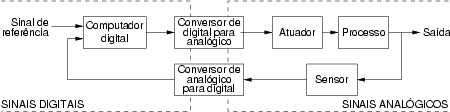
\includegraphics[scale=0.5]{tex/04-figuras/figuras/bigbitmap}
\caption{Figura \emph{pixel}-a-\emph{pixel} grande em tamanho reduzido}
\label{Fig:bigbitmapreduzida}
\end{center} \end{figure}

\begin{figure}[htbp!] \begin{center}
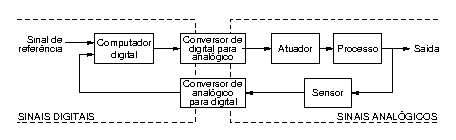
\includegraphics{tex/04-figuras/figuras/smallvetorial}
\caption{Figura vetorial pequena em tamanho natural}
\label{Fig:smallvetorial}
\vspace{6mm}
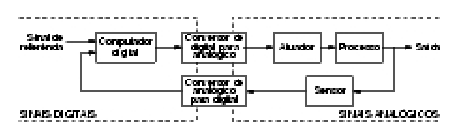
\includegraphics{tex/04-figuras/figuras/smallbitmap}
\caption{Figura \emph{pixel}-a-\emph{pixel} pequena em tamanho natural}
\label{Fig:smallbitmap}
\vspace{6mm}
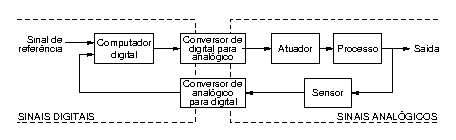
\includegraphics[width=\linewidth]{tex/04-figuras/figuras/smallvetorial}
\caption{Figura vetorial pequena em tamanho ampliado}
\label{Fig:smallvetorialampliada}
\vspace{6mm}
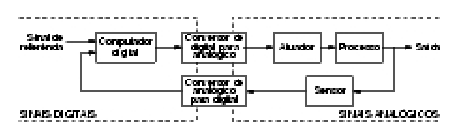
\includegraphics[width=\linewidth]{tex/04-figuras/figuras/smallbitmap}
\caption{Figura \emph{pixel}-a-\emph{pixel} pequena em tamanho ampliado}
\label{Fig:smallbitmapampliada}
\end{center} \end{figure}

Nota-se que no formato vetorial as
linhas mant�m a espessura mesmo quando se fazem
amplia��es ou redu��es. J� no formato de \emph{pixels}
as linhas ficam mais claras (cinzas, ao inv�s de pretas) ap�s as
redu��es e mais grossas ap�s as amplia��es, al�m de uma perda geral
de defini��o da imagem.

\section{Ferramentas para desenhos e esquemas}
\label{Sec:desenhos}

Existem diversas ferramentas para fazer desenhos, mas muitas delas
apenas salvam a figura gerada em formatos \emph{pixel}-a-\emph{pixel}.
No Unix, pode-se utilizar o \texttt{xfig}, que exporta imagens em
muitos formatos, inclusive nos vetoriais (PDF e EPS). Os diagramas das
figuras \ref{Fig:bigvetorial} a \ref{Fig:smallbitmapampliada} foram
desenhados e exportados no \texttt{xfig}. O arquivo fonte
correspondente � o \texttt{diagrama.fig}, no diret�rio
\texttt{figuras}.

A possibilidade de salvar figuras em modo vetorial imp�e que alguns
recursos para desenho de imagens n�o sejam oferecidos. Um deles � o
desenho a m�o-livre, j� que seria imposs�vel descrever a curva obtida
em termos de figuras geom�tricas b�sicas. Outro recurso inexistente �
o de preencher uma regi�o com uma determinada cor. Esta �ltima
limita��o muitas vezes pode ser contornada utilizando-se a no��o de
profundidade.  Por exemplo, para desenhar uma figura vazado e
preenchido de azul, pode-se desenhar a figura externa preenchido de
azul sobre o qual se desenha a figura interna preenchido de branco,
como mostram os exemplos da figura~\ref{Fig:circulo}.

\begin{figure}[htb] \begin{center}
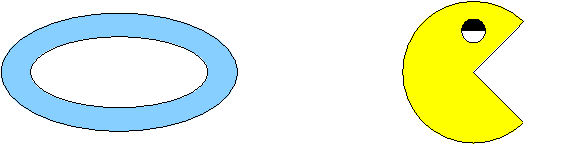
\includegraphics{tex/04-figuras/figuras/circulo}
\caption{Preenchimento de figuras utilizando diferentes profundidades}
\label{Fig:circulo}
\end{center} \end{figure}

A no��o de profundidade no \texttt{xfig} foi exaustivamente utilizada
para desenhar os s�mbolos da UFRN e do PPgEE que podem ser vistos na
p�gina de rosto deste documento. Os arquivos \texttt{xfig}
correspondentes s�o \texttt{UFRN.fig} e \texttt{PPgEE.fig}. Ela tamb�m
pode ser utilizada para mesclar imagens com figuras sint�ticas, como
na figura \ref{Fig:pensador} (veja arquivo \texttt{figuras/pensador.fig}).

\begin{figure}[htb] \begin{center}
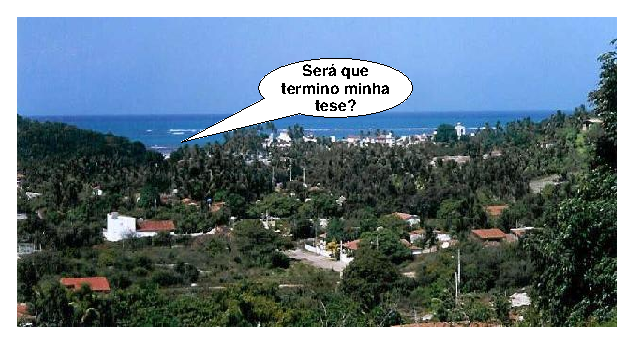
\includegraphics{tex/04-figuras/figuras/pensador}
\caption{Imagem mesclada com elementos sint�ticos}
\label{Fig:pensador}
\end{center} \end{figure}

Outra possibilidade oferecida pelo \texttt{xfig} � a inclus�o de comandos
\LaTeX\ dentro da figura. Para utilizar este recurso,
marque no \texttt{xfig} os textos que devem ser interpretados como
comandos \LaTeX\ com o \emph{flag} \texttt{special} e exporte a figura
no modo \emph{Combinado PS/Latex} ou \emph{Combinado PDF/Latex}. Veja
um exemplo na figura \ref{Fig:combinado}; note que o arquivo � inclu�do com
\verb|\input{}| e n�o com \verb|\includegraphics{}|.

% Note que foi redefinido um comando aqui no texto para ser inclu�do
% na figura. Isto � para evitar digita��o de express�es LaTeX muito
% grandes dentro do xfig
\newcommand{\formulagrande}{$\frac{G_3G_4}{1-G_3G_4H_1}$}
\begin{figure}[htb] \begin{center}
%\input{figuras/combinado.pstex_t} % Se usar latex
\input{tex/04-figuras/figuras/combinado.pdftex_t} % Se usar pdflatex
\caption{Figura incluindo comandos \LaTeX}
\label{Fig:combinado}
\end{center} \end{figure}

\section{Ferramentas para gr�ficos}
\label{Sec:graficos}

Gr�ficos devem ser gerados com aplicativos capazes de exportar o
resultado nos formatos EPS ou PDF, preferencialmente em formato
vetorial. Os conhecidos programas \emph{Scilab} e \emph{Matlab} t�m
esta capacidade. Se voc� deseja algo mais simples, a ferramenta
\textit{GNUplot} � uma das mais utilizadas no Unix para a gera��o de
gr�ficos de fun��es matem�ticas.

Uma vez gerados, gr�ficos s�o inseridos no texto tal como figuras. A
figura~\ref{fig:grafico} apresenta um gr�fico gerado atrav�s do
comando de linha \texttt{gnuplot grafico.gnuplot}. Este arquivo
\texttt{grafico.gnuplot}, que cont�m uma s�rie de comandos do
\textit{GNUplot}, est� no diret�rio \texttt{figuras}.

\begin{figure}[htbp]
\centering
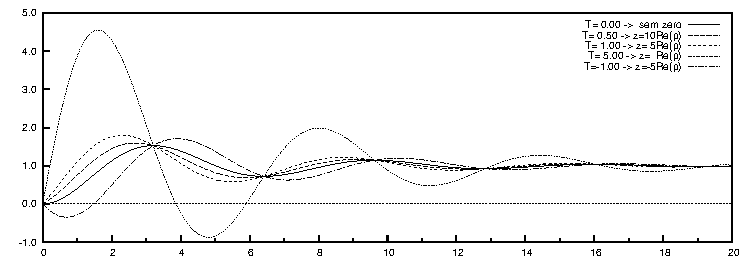
\includegraphics{tex/04-figuras/figuras/grafico}
\caption{Exemplo de gr�fico de fun��es matem�ticas}
\label{fig:grafico}
\end{figure}

\section{Conclus�es}

Ferramentas de desenho capazes de gerar a sa�da em formato vetorial
s�o mais dif�ceis de usar e parecem ser dotadas de menos recursos do
que outras que s� exportam seus resultados como imagens de
\emph{pixels}.  Isto se deve � necessidade de descrever todos os
elementos da imagem sob a forma de primitivas parametriz�veis para
permitir que elas sejam escal�veis � vontade e export�veis para
qualquer formato desejado.

Entretanto, a qualidade visual das figuras obtidas e a sua
reusabilidade � muito maior. A compara��o � aproximadamente a mesma
que a entre textos produzidos em \LaTeX\ e em editores gr�ficos. Desta
forma, na medida do poss�vel, tente conjugar a escrita do documento
\LaTeX\ com a utiliza��o de alguma ferramenta de desenho vetorial.

% LocalWords:  editadas PS


% Cap. 5 - Conclusões
%%
%% Cap�tulo 5: Conclus�es
%%

\mychapter{Conclus�es}
\label{Cap:conclusao}

O cap�tulo final depende do tipo de documento. Nas propostas de tema
deve ser apresentado de forma clara e sucinta o assunto a ser
desenvolvido e o cronograma de execu��o do trabalho. Nas teses e
disserta��es devem ser ressaltadas as principais contribui��es do
trabalho e as suas limita��es.

As contribui��es devem evitar as adjetiva��es e julgamentos de valor.
Quanto �s limita��es, n�o tenha medo de as apresentar: � muito mais
reconhecido um autor que apresenta os casos em que sua proposta n�o se
aplica do que outro que parece n�o ter consci�ncia deles.

\section{Encaderna��o}

As propostas de tema e as vers�es iniciais das teses e disserta��es
s�o impressas em lado �nico da folha e em espa�amento um e meio. Para
a encaderna��o, usa-se geralmente um m�todo simples, tal como espiral
na lateral das folhas e capa pl�stica transparente. O n�mero de c�pias
� igual ao n�mero de membros da banca e pelo menos mais uma (para o
aluno).

As vers�es finais das teses e disserta��es s�o impressas em frente e
verso e em espa�amento simples. O n�mero m�nimo de c�pias � o seguinte:
\begin{itemize}
\item 3 c�pias para o PPgEE e a UFRN.
\item 1 c�pia para cada examinador externo que participou da banca.
\item ao menos 1 c�pia para o aluno (n�o obrigat�ria).
\item 1 c�pia para o orientador (por cortesia, n�o obrigat�ria)
\end{itemize}

Para a encaderna��o, deve-se adotar uma capa r�gida de cor azul para
as disserta��es de mestrado e de cor preta para as teses de doutorado,
ambas com letras douradas. Na capa deve constar o t�tulo do
trabalho, o autor e o ano da defesa. Se poss�vel, a mesma informa��o
deve ser repetida na lombada do livro.

Para as vers�es finais, tamb�m se exige uma c�pia eletr�nica (formato
PDF) do texto, bem como outros dados. Maiores informa��es podem ser
obtidas na p�gina do PPgEE: \url{http://www.ppgee.ufrn.br/}

\section{Para saber mais}

Procure no Google, ora! Brincadeiras a parte, existem in�meros
tutoriais sobre \LaTeX\ na rede que podem dar maiores informa��es
sobre o aplicativo. Para conhecer os pacotes dispon�veis, uma op��o �
o livro \emph{The \LaTeX\ Companion} \cite{LATEX04}, popularmente
conhecido como o ``livro do cachorro''. Outras informa��es sobre
reda��o t�cnica e normas para confec��o de teses e disserta��es podem
ser encontradas em livros de Metodologia Cient�fica.


% Referências bibliogáficas (geradas automaticamente)
\addcontentsline{toc}{chapter}{Referências bibliográficas}
\bibliography{bib/bibliografia}

\appendix

%Apêndice A
%%
%% Cap�tulo 5: Conclus�es
%%

\mychapter{Informa��es adicionais}
\label{Cap:apendice}

Os ap�ndices s�o normalmente empregados para incluir informa��es
adicionais a serem eventualmente consultadas mas que n�o s�o
essenciais para a compreens�o do texto.

Evite sobrecarregar seu texto com informa��es longas e de pouco
interesse para uma primeira leitura. S�o normalmente colocados
nos ap�ndices:
\begin{itemize}
\item longas dedu��es ou demonstra��es de f�rmulas e teoremas;
\item especifica��es t�cnicas de equipamentos e descri��es de
experimentos;
\item eventuais conhecimentos dispon�veis na literatura mas que
se julga conveniente repetir no texto para facilitar a compreens�o
do leitor n�o familiarizado com a �rea;
\item outras informa��es que se julga que devam ser preservadas
mas que n�o s�o importantes no documento, tais como diagramas
esquem�ticos, algoritmos ou trechos de c�digo-fonte, folhas de
especifica��es, etc.
\end{itemize}


\end{document}
